
\section{Shape of a dusty radiative bow wave}
\label{sec:shape-dust-wave}

As an alternative to hydrodynamic or magnetohydrodynamic bow shocks,
it is possible that some observed emission arcs may be bow waves due
to the action of radiation pressure on dust grains.

\begin{figure}
  (a)\\
  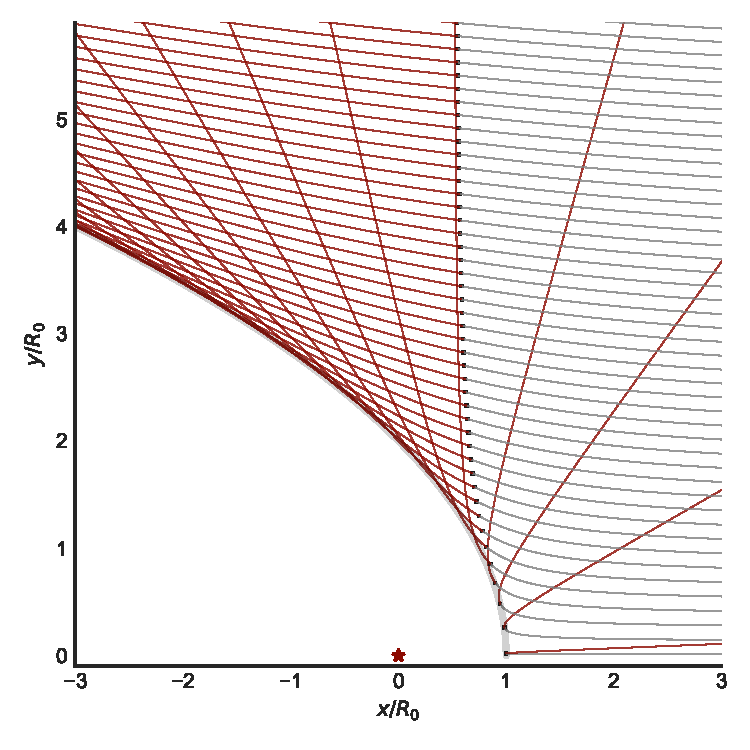
\includegraphics[width=\linewidth]{figs/dust-trajectories}
  (b)\\
  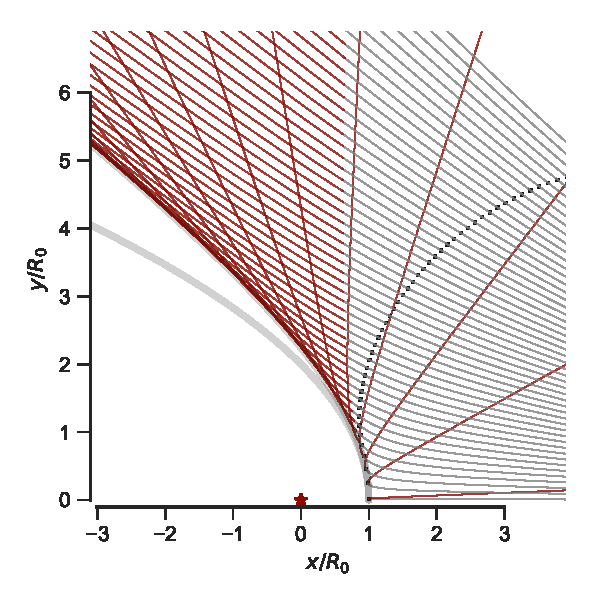
\includegraphics[width=\linewidth]{figs/dust-divergent}
  \caption[Dust grain trajectories]{Dust grain trajectories under
    influence of a repulsive central \(r^{-2}\) radiative force.
    (a)~A parallel stream of dust grains approach from the right at a
    uniform velocity and with a variety of impact parameters (initial
    \(y\)-coordinate). The central source is marked by a red star at
    the origin, and its radiative force deflects the trajectories into
    a hyperbolic shape, each of which reaches a minimum radius marked
    by a small black square.  The incoming hyperbolic trajectories are
    traced in gray and the outgoing trajectories are traced in red.
    The locus of closest approach of the outgoing trajectories is
    parabolic in shape (traced by the thick, light gray line) and this
    constitutes the inner edge of the bow wave.  (b)~The same but for
    a divergent stream of dust grains that originates from a source on
    the \(x\) axis at a distance \(D = 10 R_0\) from the origin.  In
    this case, the inner edge of the bow wave is hyperbolic and the
    parallel stream result is also shown for comparison.}
  \label{fig:dust-trajectories}
\end{figure}



\newcommand\Qp{\ensuremath{Q_{\text{p}}}}
\newcommand{\grain}{\ensuremath{_{\text{d}}}}
\newcommand{\xsec}{\ensuremath{\sigma\grain}}
\newcommand\frad{\ensuremath{f_{\text{rad}}}}
\newcommand\thm{\ensuremath{\theta_{\text{m}}}}
A dust grain of geometrical cross-section \(\xsec\) situated a
distance \(R\) from a point source of radiation with luminosity \(L\)
will experience a repulsive, radially directed radiative force
\citep[e.g.,][]{Spitzer:1978a}
\begin{equation}
  \label{eq:dust-rad-force}
  \frad = \frac{\xsec \Qp L} {4 \pi R^2 c} e^{-\tau}
\end{equation}
where \Qp{} is the frequency-averaged\footnote{%
  Frequency averages of any quantity \(x\) should be understood as
  weighted by the attenuated source spectrum:
  \(\langle x \rangle_\nu = (L \, e^{-\tau})^{-1} \int_0^\infty x(\nu)\, L_\nu \, e^{-\tau_\nu} \, d\nu
  \).  } %
radiation pressure efficiency\footnote{%
  For absorption efficiency \(Q_{\text{abs}}\), scattering efficiency
  \(Q_{\text{scat}}\), and asymmetry parameter (mean scattering
  cosine) \(g\), we have
  \(\Qp = Q_{\text{abs}} + (1 - g) Q_{\text{scat}}\)
  \citep[e.g., \S~4.5 of][]{Bohren:1983a}.} %
of the grain, \(c\) is the speed of light, and \(\tau\) is the
frequency-averaged optical depth between the source and the grain.
For simplicity, we will consider only the optically thin case,
\(\tau \to 0\).

\subsection{Gas-free bow wave}
\label{sec:gas-free-bow}


If \(\frad\) is the only force experienced by the grain, then it will
move on a \textit{ballistic} trajectory, determined by its initial
speed at large distance, \(v_\infty\), and its impact parameter, \(b\).
For \(b = 0\), the grain radially approaches the source with initial
radial velocity \(-v_\infty\), which is decelerated to zero at the distance
of closest approach, \(R_0\), given by energy conservation:
\begin{equation}
  \label{eq:dust-r0}
  R_0 = \frac{\xsec \Qp L} {2 \pi c m\grain v_\infty^2} \ ,
\end{equation}
where \(m\grain\) is the grain mass.  The grain then turns round and
recedes from the source along the same radius, reaching a velocity of
\(+v_\infty\) at large distance.  For \(b > 0\), the trajectory,
\(R\grain(\theta; b)\), is found\footnote{%
  The problem is formally identical to that of Rutherford scattering,
  or (modulo a change of sign) planetary orbits.  The method of
  solution (via introduction of a centrifugal potential term and
  reduction to a 1-dimensional problem) can be found in any classical
  mechanics text \citep[e.g.,][\S~14]{Landau:1976a}.} %
to be hyperbolic, characterized by an eccentricity,
\(\varepsilon = \bigl( 1 + 4 b^2 / R_0^2\bigr)^{1/2}\), and polar angle of
closest approach, \(\thm = \cos^{-1} \varepsilon^{-1}\).  The trajectory is
symmetrical about \(\thm\) and can be written as
\begin{equation}
  \label{eq:dust-r-theta}
  \frac{R\grain(\theta; b)} {R_0} = 
  \frac{ \tfrac12 \bigl( \varepsilon^2 - 1 \bigr)} {\varepsilon \cos(\theta - \thm) - 1} \ , 
\end{equation}
with a total deflection angle of \(2 \thm\), which is equal to
\(90^\circ\) when \(b = 0.5 R_0\).

\subsubsection{Parallel dust stream}
\label{sec:dust-parallel}

If the incoming dust grains initially travel along parallel
trajectories with varying \(b\), but the same \(v_\infty\), then deflection
by the radiative force will form a bow wave around the radiation
source, as shown in Figure~\ref{fig:dust-trajectories}.  However, the
inner edge of the bow wave, \(R_{\text{in}}(\theta)\) is not given by the
closest approach along individual trajectories, \(R\grain(\thm; b)\),
but instead must found by minimizing \(R\grain(\theta; b)\) over all
\(b\) for each value of \(\theta\), which yields
\begin{equation}
  \label{eq:dust-r-in}
  \frac{R_{\text{in}}(\theta)} {R_0} = \frac{2}{1 + \cos\theta} \ .
\end{equation}
This is the polar form of the equation for the confocal parabola,
which we have already discussed in detail in \S~\ref{sec:conic} and
Appendix~\ref{app:parabola}.  Its planitude and alatude are
\(\Gamma = \Lambda = 2\) and these are unchanged under projection at any
inclination.


\subsubsection{Divergent dust stream}
\label{sec:dust-divergent}

If the dust grains are assumed to originate from a second point
source, located at a distance \(D\) from the radiation source, then
the incoming stream will be divergent instead of plane parallel.  The
individual streamlines are not affected by this change and are still
described by equation~\eqref{eq:dust-r-theta}, except that the
trajectory axes for \(b > 0\) are no longer aligned with the global
symmetry axis, so we must make the substitution
\(\theta \to \theta + \theta_1(b)\), where \(\sin \theta_1 = b / D\) (see
Fig.~\ref{fig:crw-schema}). We parametrize the degree of divergence as
\(\mu = R_0 / D\) and, as before, \(R\grain(\theta + \theta_1(b, \mu); b)\) is
minimized over all trajectories to find the shape of the bow wave's
inner edge.  This time, the result is a confocal hyperbola:
\begin{equation}
  \label{eq:dust-divergent-r-in}
  \frac{R_{\text{in}}(\theta; \mu)} {R_0} = \frac{1 + \varepsilon_\mu}{1 + \varepsilon_\mu\cos\theta} \ ,
\end{equation}
where the eccentricity is (to first order in \(\mu\))
\( \varepsilon_\mu = (1 - 2\mu)^{-1}\).  An example is shown in
Figure~\ref{fig:dust-trajectories} for \(\mu = 0.1\).  Unsurprisingly,
the resulting bow shape is more open than in the parallel stream case,
increasingly so with increasing \(\mu\).  The planitude and alatude are
both equal: \(\Pi = \Lambda = 1 + \varepsilon_\mu\).

\newcommand\drag{\ensuremath{_{\text{drag}}}}
\newcommand{\gas}{\ensuremath{_{\text{gas}}}}
\newcommand{\drift}{\ensuremath{_{\text{drift}}}}
\newcommand\soundspeed{\ensuremath{c_{\text{s,gas}}}}


\begin{figure}
  \centering
  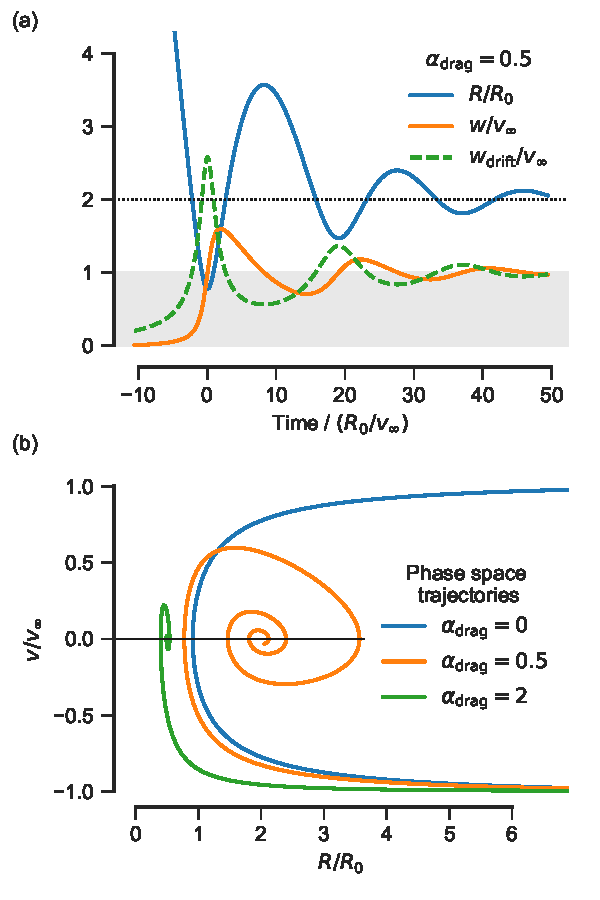
\includegraphics[width=\linewidth]{figs/dust-coupling-1d}
  \caption{Dust-gas coupling for an on-axis (purely radial)
    trajectory.  (a)~Grain radial position, \(R/R_0\), gas--grain
    velocity difference, \(w/v_\infty\), and local asymptotic drift
    velocity, \(w\drift/v_\infty\), versus time for
    \(\alpha\drag = 0.5\).  The behavior is typical of the dynamics of a
    damped harmonic oscillator. (b)~Phase space (position, velocity)
    trajectories for \(\alpha\drag = 0\), 0.5, and 2. All trajectories
    begin in the lower right corner and evolve in a clockwise
    direction. For \(\alpha\drag > 0\), the grain spirals in on the point
    \((x, u) = (\alpha\drag^{-1}, 0)\).}
  \label{fig:dust-coupling-1d}
\end{figure}

\begin{figure*}
  \centering
  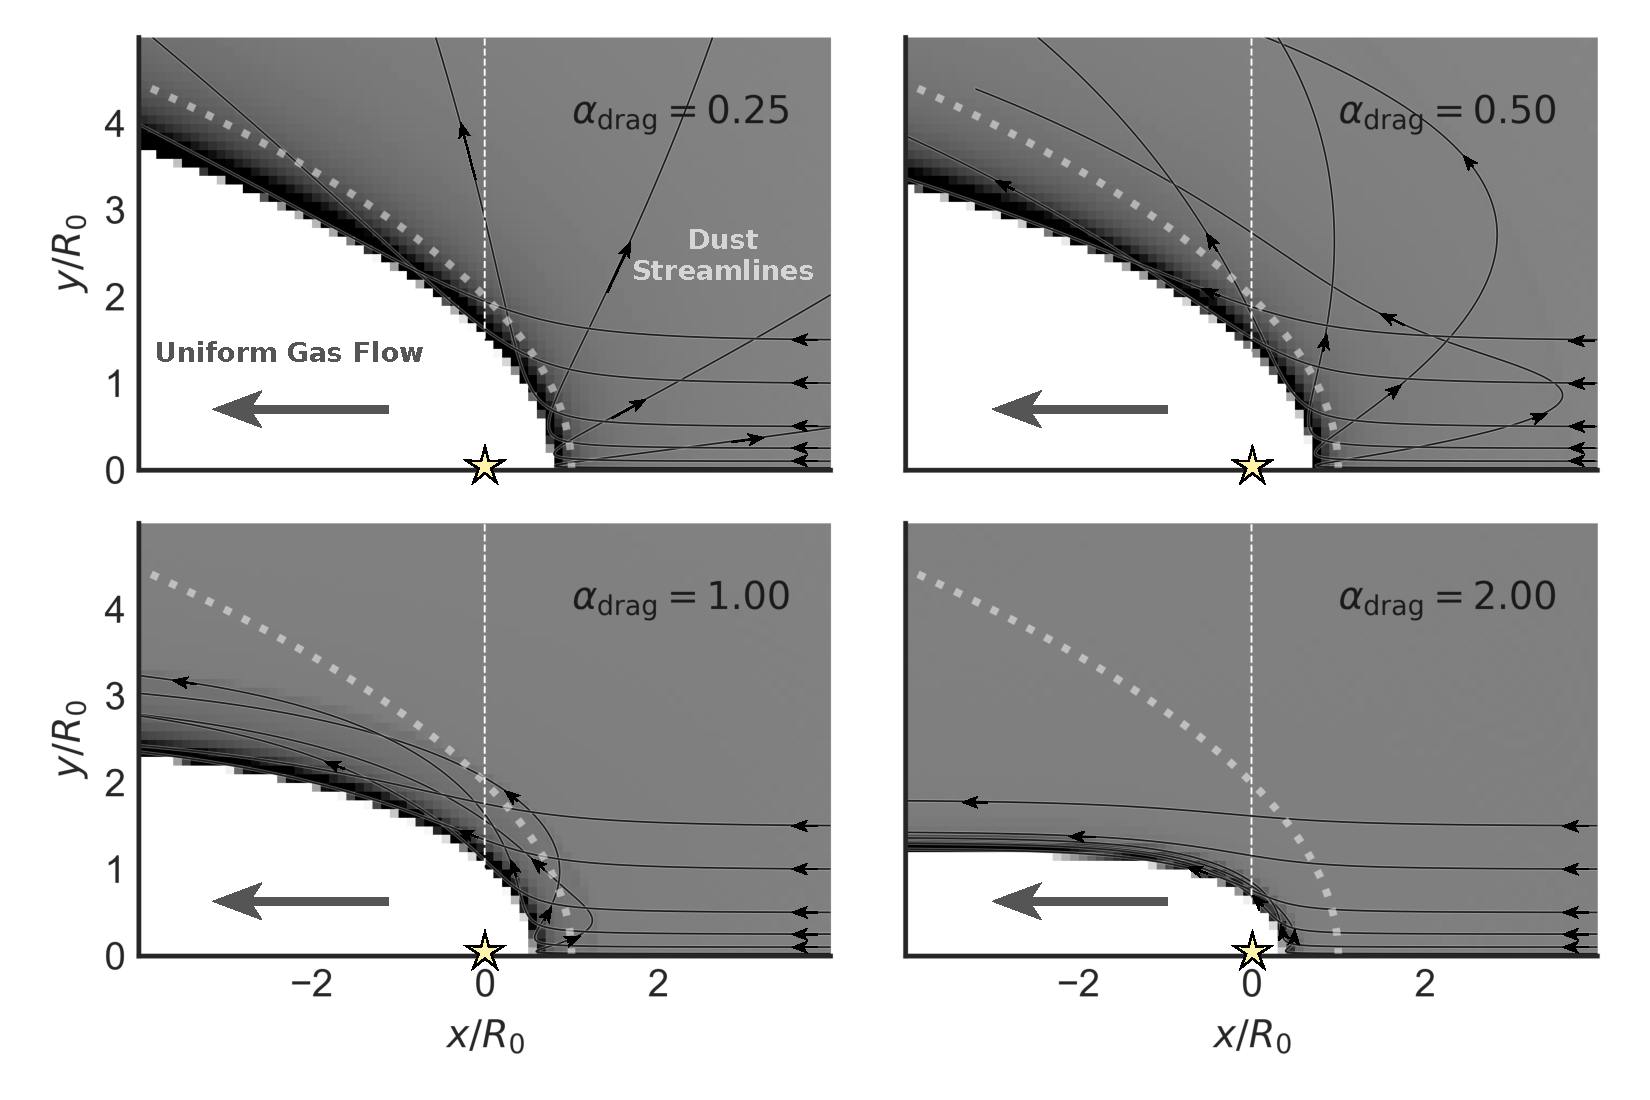
\includegraphics[width=\linewidth]{figs/dust-couple-stream-annotate}
  \caption{Dust grain trajectories under influence of gas drag in
    addition to a repulsive central radiative force.  The dust
    streamlines are shown as black lines with arrows and the dust
    density as a linear gray scale, with maximum (black) of twice the
    ambient dust density.  Results are shown for four values of the
    drag parameter (see text): \(\alpha_\text{drag} = 0.25\), \(0.5\),
    \(1.0\), and \(2.0\). The shape of the bow wave for the drag-free
    case (Fig.~\ref{fig:dust-trajectories}) is shown by the thick
    dotted line.  Faint patterns visible in the density away from the
    bow wave are numerical aliasing artefacts caused by sparse
    sampling of the streamlines in the low density regions.}
  \label{fig:dust-wave-coupling}
\end{figure*}


\subsection{Bow wave with gas drag}
\label{sec:bow-wave-drag}

More realistically, a grain will also be subject to a drag force,
\(f\drag\), due to its relative motion with respect to gas or plasma
particles. If the gas density, velocity, and sound speed are
\(\rho\gas\), \(v\gas\), and \(\soundspeed\), then a grain with velocity
\(v\grain\) will experience a drag force that is directed opposite to
the relative velocity, \(\bm{w} = \bm{v}\grain - \bm{v}\gas\).  In the
supersonic limit, \(w \equiv \abs{\bm{w}} \gg \soundspeed\), the magnitude of
the force is
\begin{equation}
  \label{eq:dust-fdrag}
  \abs{f\drag} \approx Q\drag \xsec \rho\gas w^2 \ ,
\end{equation}
where \(Q\drag\) is an efficiency factor (which may be smaller or
greater than unity) that accounts for details such as sticking
probability and the boost in cross section due to the Coulomb force
when a charged grain interacts with an ionized plasma
\citep{Draine:1979a}.  We neglect the back reaction of the dust on the
gas motion and assume a uniform background gas flow that is perfectly
coupled to the incoming dust stream at large radii.  So, for the
parallel stream case, we have \(\bm{v}\gas = -v_\infty \uvec{x}\) everywhere.

Considering the incoming flow on the symmetry axis, at each radius
there is an asymptotic gas--grain drift speed, \(w\drift\), for which
the radiative and drag forces exactly cancel, \(f\drag = -\frad\),
yielding
\begin{equation}
  \label{eq:dust-wdrift}
  w\drift = \left( \frac{\Qp L} {4\pi c Q\drag \rho\gas R^2} \right)^{1/2} \ .
\end{equation}
Any deviation of \(w\) from \(w\drift\) produces unbalanced forces
that tend to restore \(w \to w\drift\), although the grain inertia means
that this will not happen instantaneously, so that if \(w\drift\)
varies rapidly along a streamline, then changes in \(w\) will lag
behind.  We define a dimensionless coupling coefficient,
\(\alpha\drag\), to be the speed of the incoming stream in units of the
drift velocity at the radiative turn-around radius:
\begin{equation}
  \label{eq:dust-alpha}
  \alpha\drag \equiv \frac{v_\infty} {w\drift(R_0)} = \left(
    Q\drag \frac{R_0 / a\grain} {\rho\grain / \rho\gas}
  \right)^{1/2} \ ,
\end{equation}
where we have used equation~\eqref{eq:dust-r0} and suppressed a
grain-shape dependent geometric factor of order unity.  If
\(\alpha\drag \ll 1\), then \(w\drift \gg v_\infty\) out to several times the
turn-around radius, so the radiation field has no difficulty in
effectively decoupling the grain from the gas and producing the
velocity difference that is required to turn the grain around and
expel it towards the direction whence it came (\(w = 2 v_\infty\)).
However, for non-zero \(\alpha\drag\) the \(R^{-1}\) dependence of
\(w\drift\) (eq.~\eqref{eq:dust-wdrift}) means that the grain will
\textit{re-couple} to the inflowing gas stream around a radius
\(\approx R_0 / \alpha\drag \) and be swept back in again for another approach to
the source.  A further effect of increasing \(\alpha\drag\) is that the
grain penetrates closer to the star on its initial approach, thanks to
the tail wind provided by the gas flow.  Both these behaviors are
illustrated in Figure~\ref{fig:dust-coupling-1d}, where the inertial
lag of \(w\) behind \(w\drift\) means that the phase space trajectory
(panel b) is a spiral, which converges on the stagnation point
\((R, v) = (R_0 / \alpha\drag, 0)\). The cases \(\alpha\drag = 0.5\) and
\(\alpha\drag = 2\) are shown, and it can be seen that with larger
\(\alpha\drag\) the oscillations about the stagnation radius are
significantly damped.

However, this description only applies to grains with impact
parameter, \(b\), that is exactly zero.  Even a very small finite
\(b\) means that \(\frad\) has a component perpendicular to the axis,
which pushes the grain to the side and means that, after re-coupling,
its second approach is at a much larger impact parameter than its
first, so it is dragged around the wings of the bow wave before it can
bounce in and out more than twice.  This is illustrated in
Figure~\ref{fig:dust-wave-coupling}, which shows grain trajectories
and the resulting dust density structure, calculated from numerical
integration of equations~\eqref{eq:dust-rad-force}
and~\eqref{eq:dust-fdrag} in 2-D cylindrical coordinates.  Results are
shown for a range of coupling parameters, \(\alpha\drag\).  The
\(\alpha\drag = 0.25\) case appears qualitatively similar to the no-drag
case shown in Figure~\ref{fig:dust-trajectories}a, except that the
inner edge of the bow wave has been shifted to a smaller radius.
Recoupling of the outgoing streamlines to the gas flow does occur
eventually, but on length scales larger than shown in the figure. The
\(\alpha\drag = 0.5\) case shows the oscillating trajectories discussed
above for those grains that come in with a small initial impact
parameter.  In the \(\alpha\drag = 1.0\) case, the oscillating trajectories
are more confined, forming a thick shell around \(R_0\).  In the
\(\alpha\drag = 2.0\) case, the shell is much thinner and concentrated at
the inner rim.  As \(\alpha\drag\) increases, the oscillations are damped
further so that the stagnation radius \(R_0 / \alpha\drag\) becomes a good
approximation to the apex radius of the density wave.  All the cases
illustrated are for a parallel incident stream, but a divergent stream
gives qualitatively similar behavior.  We propose the term
\textit{dragoid} for the 3-dimensional shapes of the bow waves, found
by rotating results such as Figure~\ref{fig:dust-wave-coupling} about
the symmetry axis.


\subsection{Applicability of the bow wave models}
\label{sec:dust-applicability}

The apex turn-around radius, \(R_0\), of the bow wave depends on the
grain properties via the combination \(\xsec \Qp / m\grain\).  For
grains of size \(a\grain\) and internal density \(\rho\grain\), we have
\(\xsec / m\grain \approx (a\grain \rho\grain)^{-1}\).  For radiation with
wavelength smaller than the grain size, \(\lambda < a\grain\), the
efficiency is \(\Qp \sim 1\), whereas for \(\lambda > a\grain\) it is
\(\Qp \sim a\grain/\lambda\).  Therefore, we would expect \(R_0\) to be almost
independent of grain size for small grains, but to vary as
\(R_0 \propto a\grain^{-1}\) for large grains, where small/large is relative
to the peak wavelength of the radiation source.  In principle, a
polydisperse population of grains could produce a blurring of the
observed bow wave, but only if large grains contribute significantly
to the dust emission.


\TODO{Variation of \(\alpha\drag\) with grain size, charged grains.}

\TODO{Lorentz force, Larmor radius}

\TODO{Back-reaction on gas, \(\alpha\drag \to \infty\), recovery of drag-free
  results but with increased effective grain mass.}

\section{Apparent shapes of projected dragoids}
\label{sec:dust-wave-apparent}

\begin{figure}
  \centering
  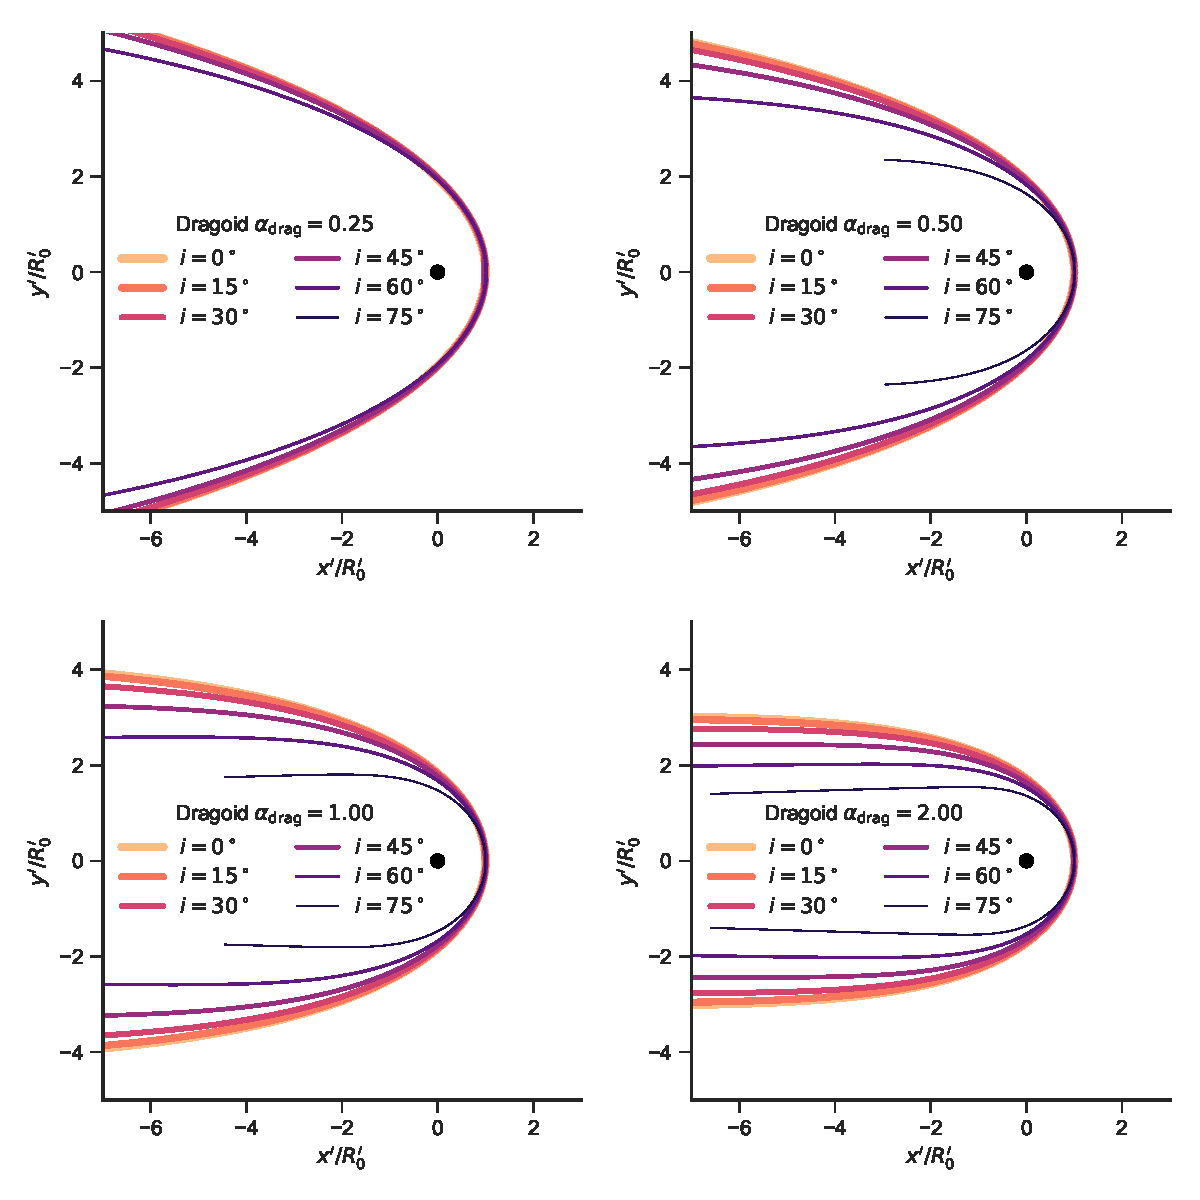
\includegraphics[width=\linewidth]{figs/test_xyprime_dragoid}
  \caption{Plane-of-sky shapes for dragoids.}
  \label{fig:dragoid-xy-prime}
\end{figure}


\begin{figure}
  \centering
  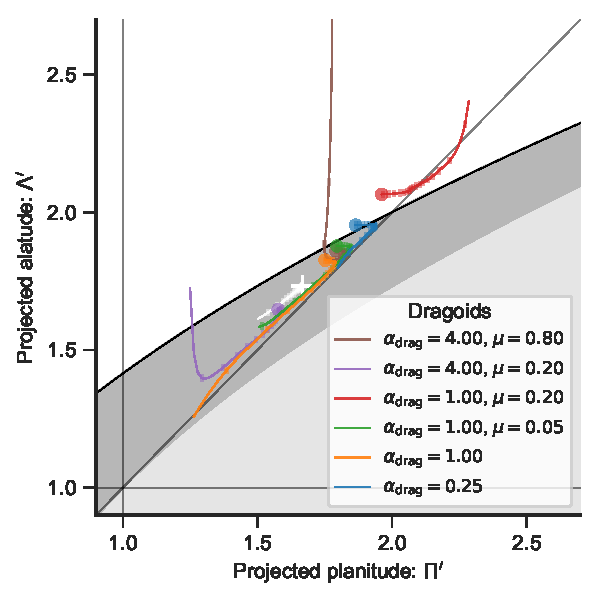
\includegraphics[width=\linewidth]{figs/dragoid-R90-vs-Rc}
  \caption{Diagnostic diagram for dragoids}
  \label{fig:dragoid-Rc-R90}
\end{figure}

%%% Local Variables:
%%% mode: latex
%%% TeX-master: "quadrics-bowshock"
%%% End:
